\subsection{Background}
Wavelets are mathematical tools that are often used in the context of signal processing. They were introduced by Alfréd Haar in 1909\cite{haar} and wavelet theory was later expanded by multiple mathematicians, including Stéphane Mallat and Ingrid Daubechies. Wavelet transforms can be viewed as a generalization of Fourier transforms. While the latter only contain frequency information, the former capture information about location in time as well. Both continous and discrete wavelet transforms (DWT) admit an inverse transform.

DWTs and inverse discrete wavelet transforms (IDWT) are often used in the contexts of computer vision\cite{wavelet_application_4} and image processing\cite{wavelet_application_1}\cite{wavelet_application_2}, both for image compression and denoising\cite{wavelet_application_3}. In particular, the 5/3 and 9/7 wavelet transforms are used in the JPEG 2000 standard, for reversible and irreversible compression respectively, achieving both a higher compression rate and higher image quality over JPEG.

In the simplest implementation of a DWT, a signal is convolved with a low-pass and a high-pass filter. A more efficient implementation which uses a lifting scheme was proposed by Wim Sweldens\cite{lifting}. While 1D DWTs have a computational complexity of $O(n)$, 2D DWTs require computing the DWT of each row and each column of the input and are often the main computational kernel in applications that use them. As such, multiple works that focus on optimizing DWT computations have been proposed\cite{wavelet_fast_1}\cite{wavelet_fast_2}\cite{wavelet_fast_3}\cite{wavelet_fast_4}.

The coefficients of the 2D DWT of an image can be divided into four sets, based on which pixels contain low or high-passed data. These sets are denoted as LL, HL, LH and HH and can be visualized as an image like in Figure \ref{fig:wavelet_2d}, where the top-left quadrant contains the data of the LL set.

\subsection{Implemented features}
We implemented two versions of the 1D and 2D 9/7 DWT and IDWT, both using lifting. The first version was adapted from C code by Gregoire Pau\cite{gregoire_pau} and rewritten in modern C++. The second implementation was developed following the descriptions in \cite{Daubechies} and \cite{wavelet_fast_1}. Since the reported articles do not specify how to treat the first and last value in the high and low passed sequences, the same approach as the previously mentioned implementation was used. The two DWT implementations do not provide identical transforms for the same sequences. Due to the lack of complete and reliable documentation, we were unable to establish which implementation corresponds to the real 9/7 DWT, as both implementations provide valid results in their applications to image processing.

As a proof of concept, we used the 2D algorithms for simple image processing applications. An instance of \texttt{DaubechiesWaveletTransform97} was applied to an example image. The resulting coefficients where then mapped into the range [0, 255] using an affine map and interpreted as pixel values, obtaining the results in Figure \ref{fig:wavelet_2d}. The test case is aimed at reproducing \cite{castle}, where the image was further processed for displaying purposes, achieving more visible details in the darker quadrants. The test shows that the LL quadrant contains an image similar to the original one. Despite the fact that other quadrants are dark, zooming it one can make out the sharp edges in the original image. This example shows one of the advantages of DWTs over DFTs, i.e. the ability to extract information about sharp changes in an image, which the human eye is very susceptible to.

\begin{figure}[h]
    \centering
    \subfigure[Original]{\label{fig:a}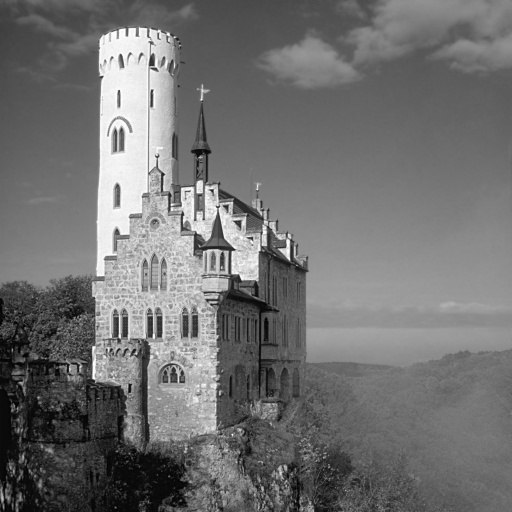
\includegraphics[width=35mm]{image/castle_original}}
    \subfigure[1-level DWT]{\label{fig:b}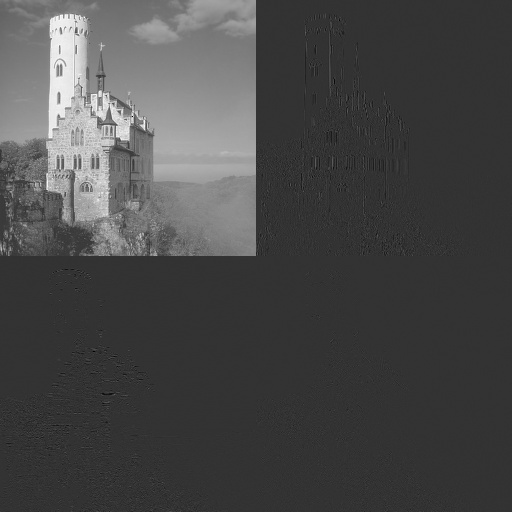
\includegraphics[width=35mm]{image/castle_level1}}
    \subfigure[2-level DWT]{\label{fig:b}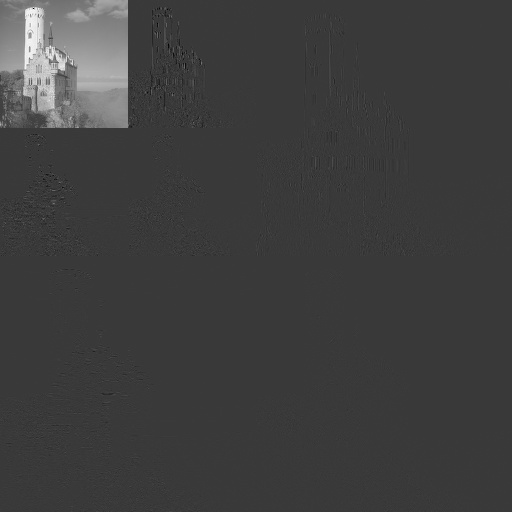
\includegraphics[width=35mm]{image/castle_level2}}
    \caption{Multi level DWT applied to an example image.}
    \label{fig:wavelet_2d}
\end{figure}

\textcolor{green}{Insert an image about denoising}

Wavelet code was written with the objectives of readability and expandability, but no in-depth performance analysis was performed. Additionally, the 2D algorithms use conditional OpenMP parallelization over the rows and columns of the input. While the DWT and IDWT implementations of \texttt{Daubechies\-Wavelet\-Transform\-97} are parallelizable as well, parallelization was avoided, as consumer-grade architectures have a number of processors that is far lower than the amount that would benefit from this nested parallelization.

\subsection{Code}
Most wavelet-related functionalities are declared in \texttt{Wavelet\-Transform.hpp} and implemented in \texttt{Wavelet\-Transform.cpp}. An abstract class \texttt{Wavelet\-Transform\-Algorithm} with two virtual methods \texttt{direct\-Transform} and \texttt{inverse\-Transform} is declared. Two classes representing the two 1D DWT algorithms inherit from it, overriding its methods. Moreover, a \texttt{Two\-Dimensional\-Wavelet\-Transform\-Algorithm} class is declared. Said class is passed a unique pointer to a \texttt{Wavelet\-Transform\-Algorithm} as a constructor argument and specifies two public methods for performing a 2D DWT and IDWT using the provided 1D algorithm.

\texttt{Grayscale\-Image.cpp} contains the definitions of two more wavelet-related methods: \texttt{wavelet\-Transform} and \texttt{denoise}, used to apply a 2D DWT to the image and visualize the result and to denoise an image respectively.

Finally, wavelet-related functionalities are used in \texttt{wavelet\_main.cpp}.